\subsection{Montages}
Pour effectuer l'étude du matériau considéré, on mesure la résistance de l'échantillon grâce à la technique de mesure 4 pointes.
On mesure en même temps la résistance d'une sonde de température qui a été étalonnée.
Donc, à partir de ces données on peut en déduire la conductivité de l'échantillon en fonction de la température.

Nous avons commencé avec une mesure sur un conducteur (le cuivre) pour partir sur quelque chose de simple.
La tendance attendue pour Cu semblait être facile à obtenir (la résistance d'un métal augmente linéairement avec la température), donc nous avons débuté avec ce métal.

Puis nous avons voulu effectuer une mesure sur un semi-conducteur, nous avons donc commandé deux wafers de silicium (dopés N et P), et poursuivi les mesures avec ces échantillons.

\subsubsection{Schémas}

\subsubsection{Photos}

Voici quelques photos du montage de base : Figures \ref{photo1}, \ref{photo2}, \ref{photo3}, avec les deux multimètres \emph{Fluke 8840A}, les 4 pointes de mesure, placées dans un support que nous avons percé nous-mêmes dans une place de polystyrène, tenu grâce à une potence. Un autre porte échantillon sert à placer la sonde de température, et l'échantillon étudié est posé sur un élévateur, pour pouvoir plus facilement faire le contact avec les 4 pointes.

\begin{figure}[!t]
  \begin{center}
		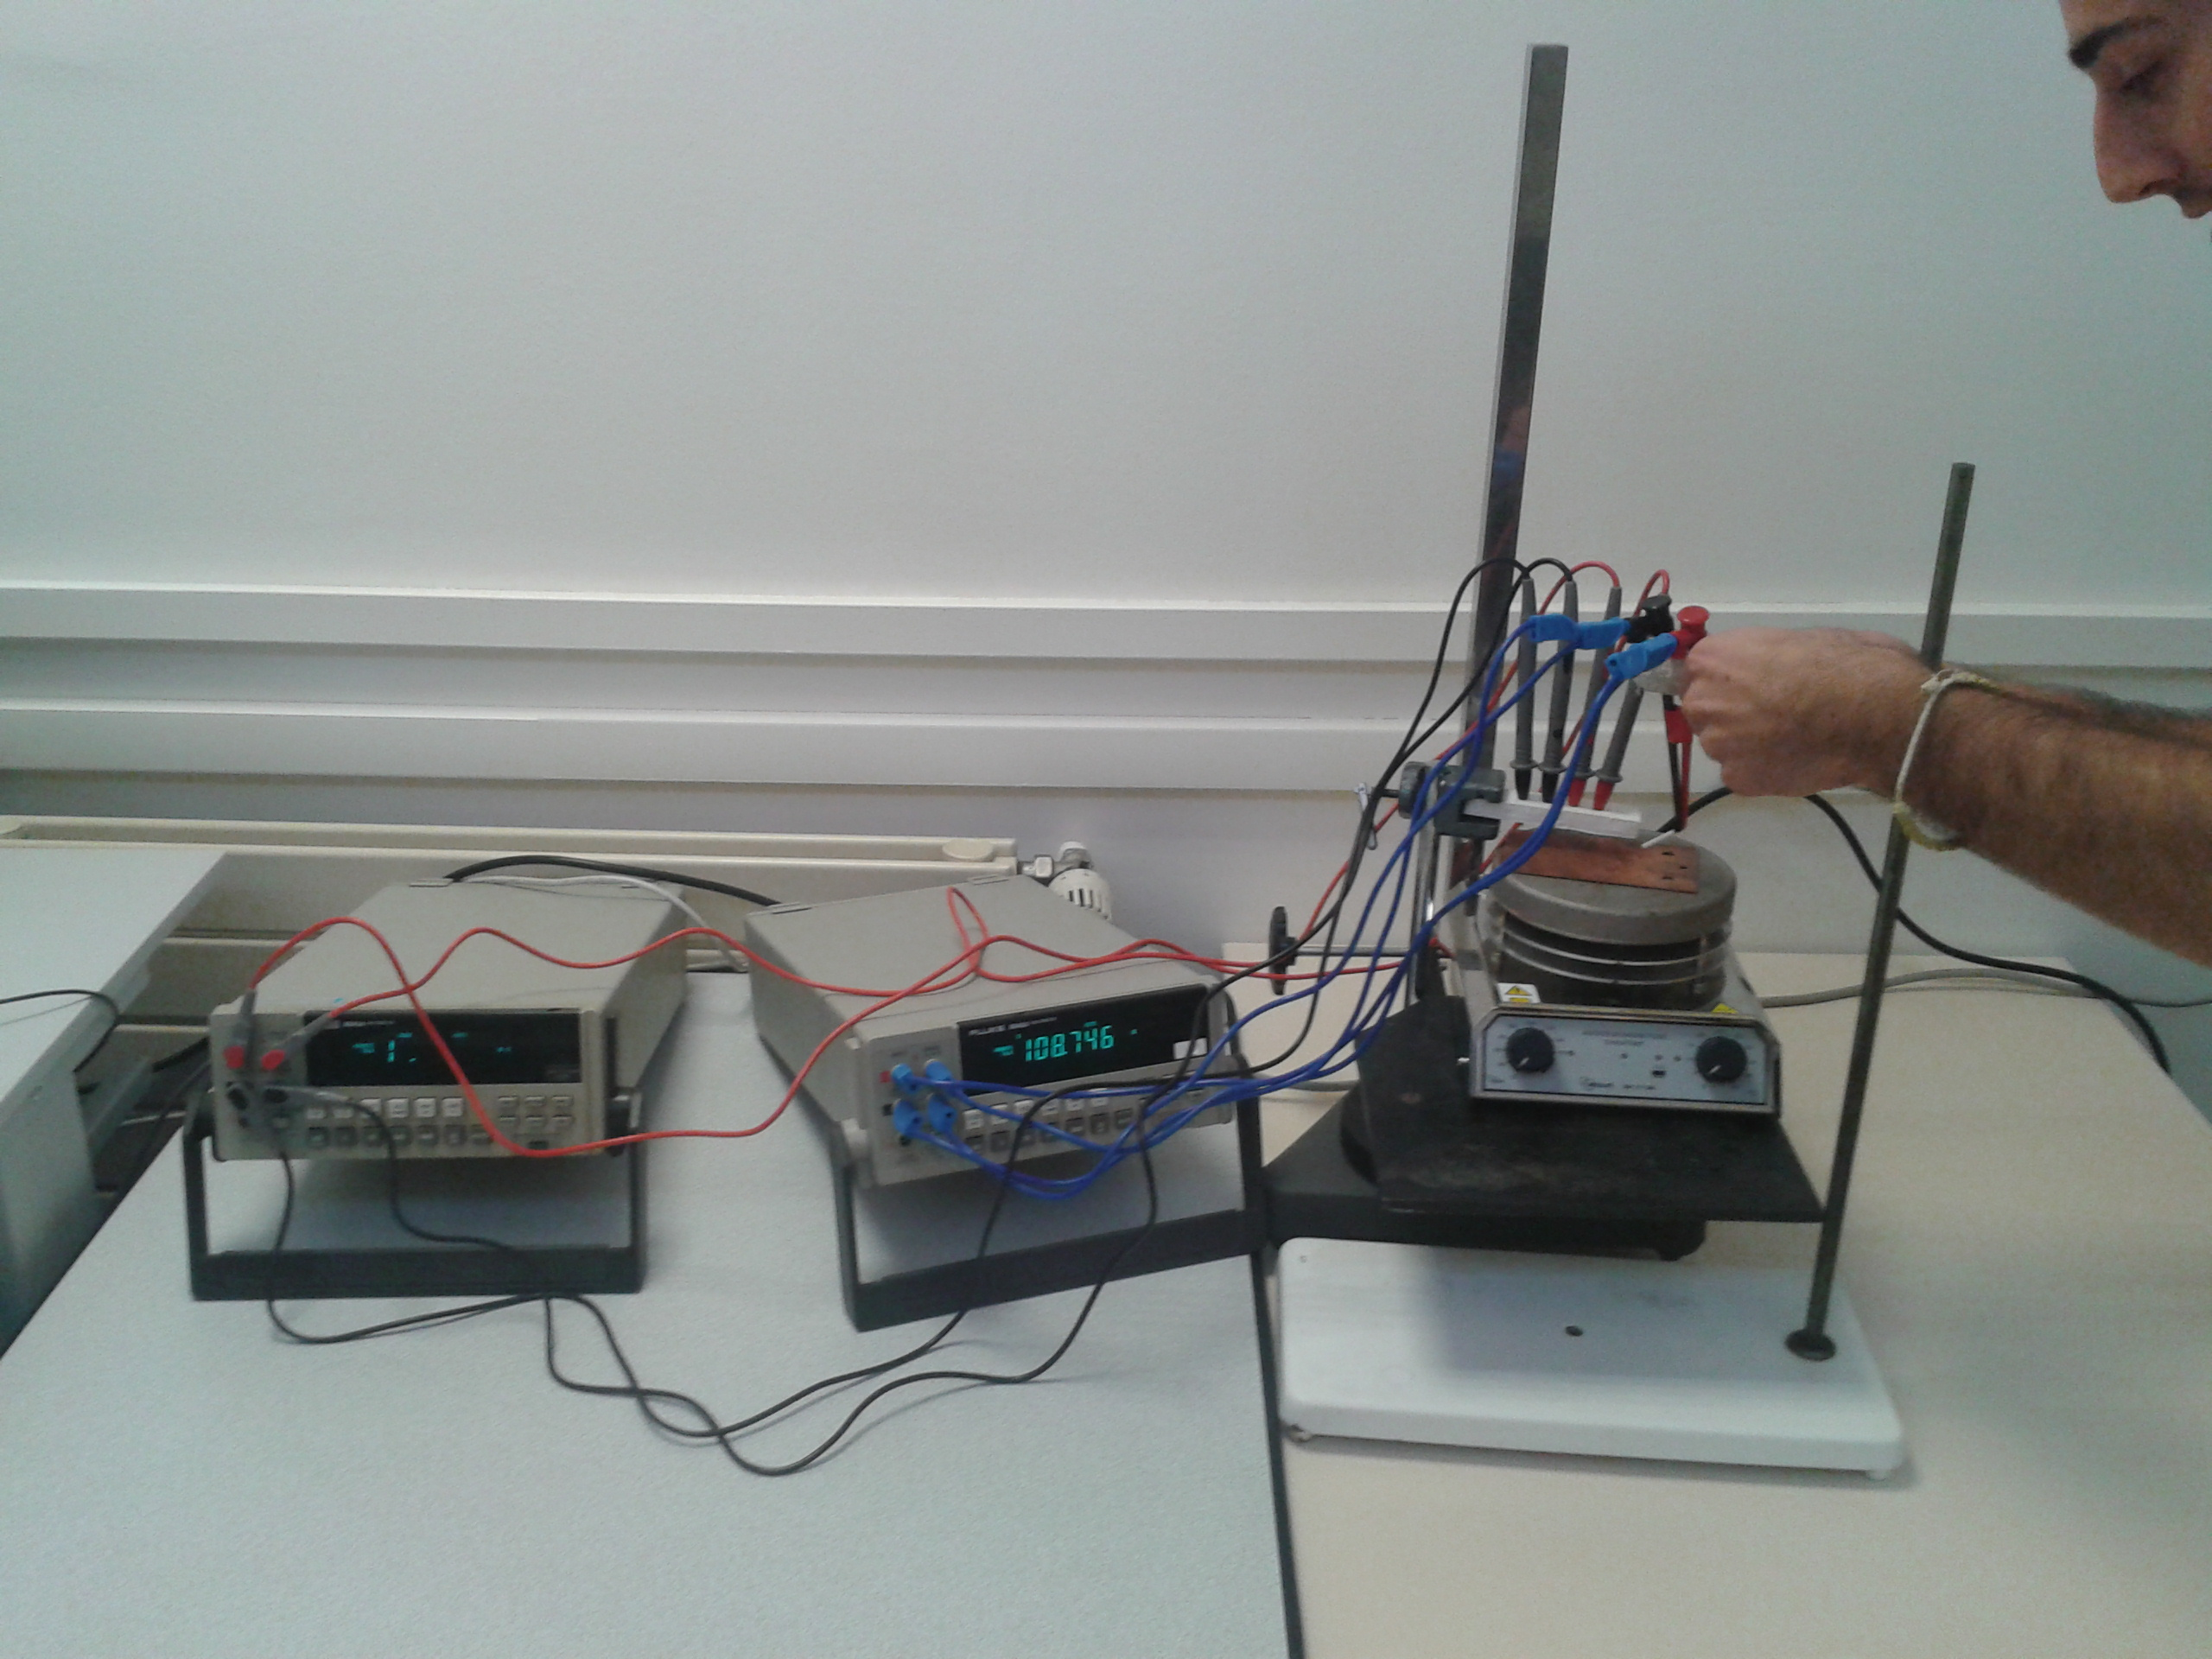
\includegraphics[width=10cm]{./images/photo1.jpg}
		\caption{Montage général}
		\label{photo1}
	\end{center}
\end{figure}
\begin{figure}[!b]
  \begin{center}
		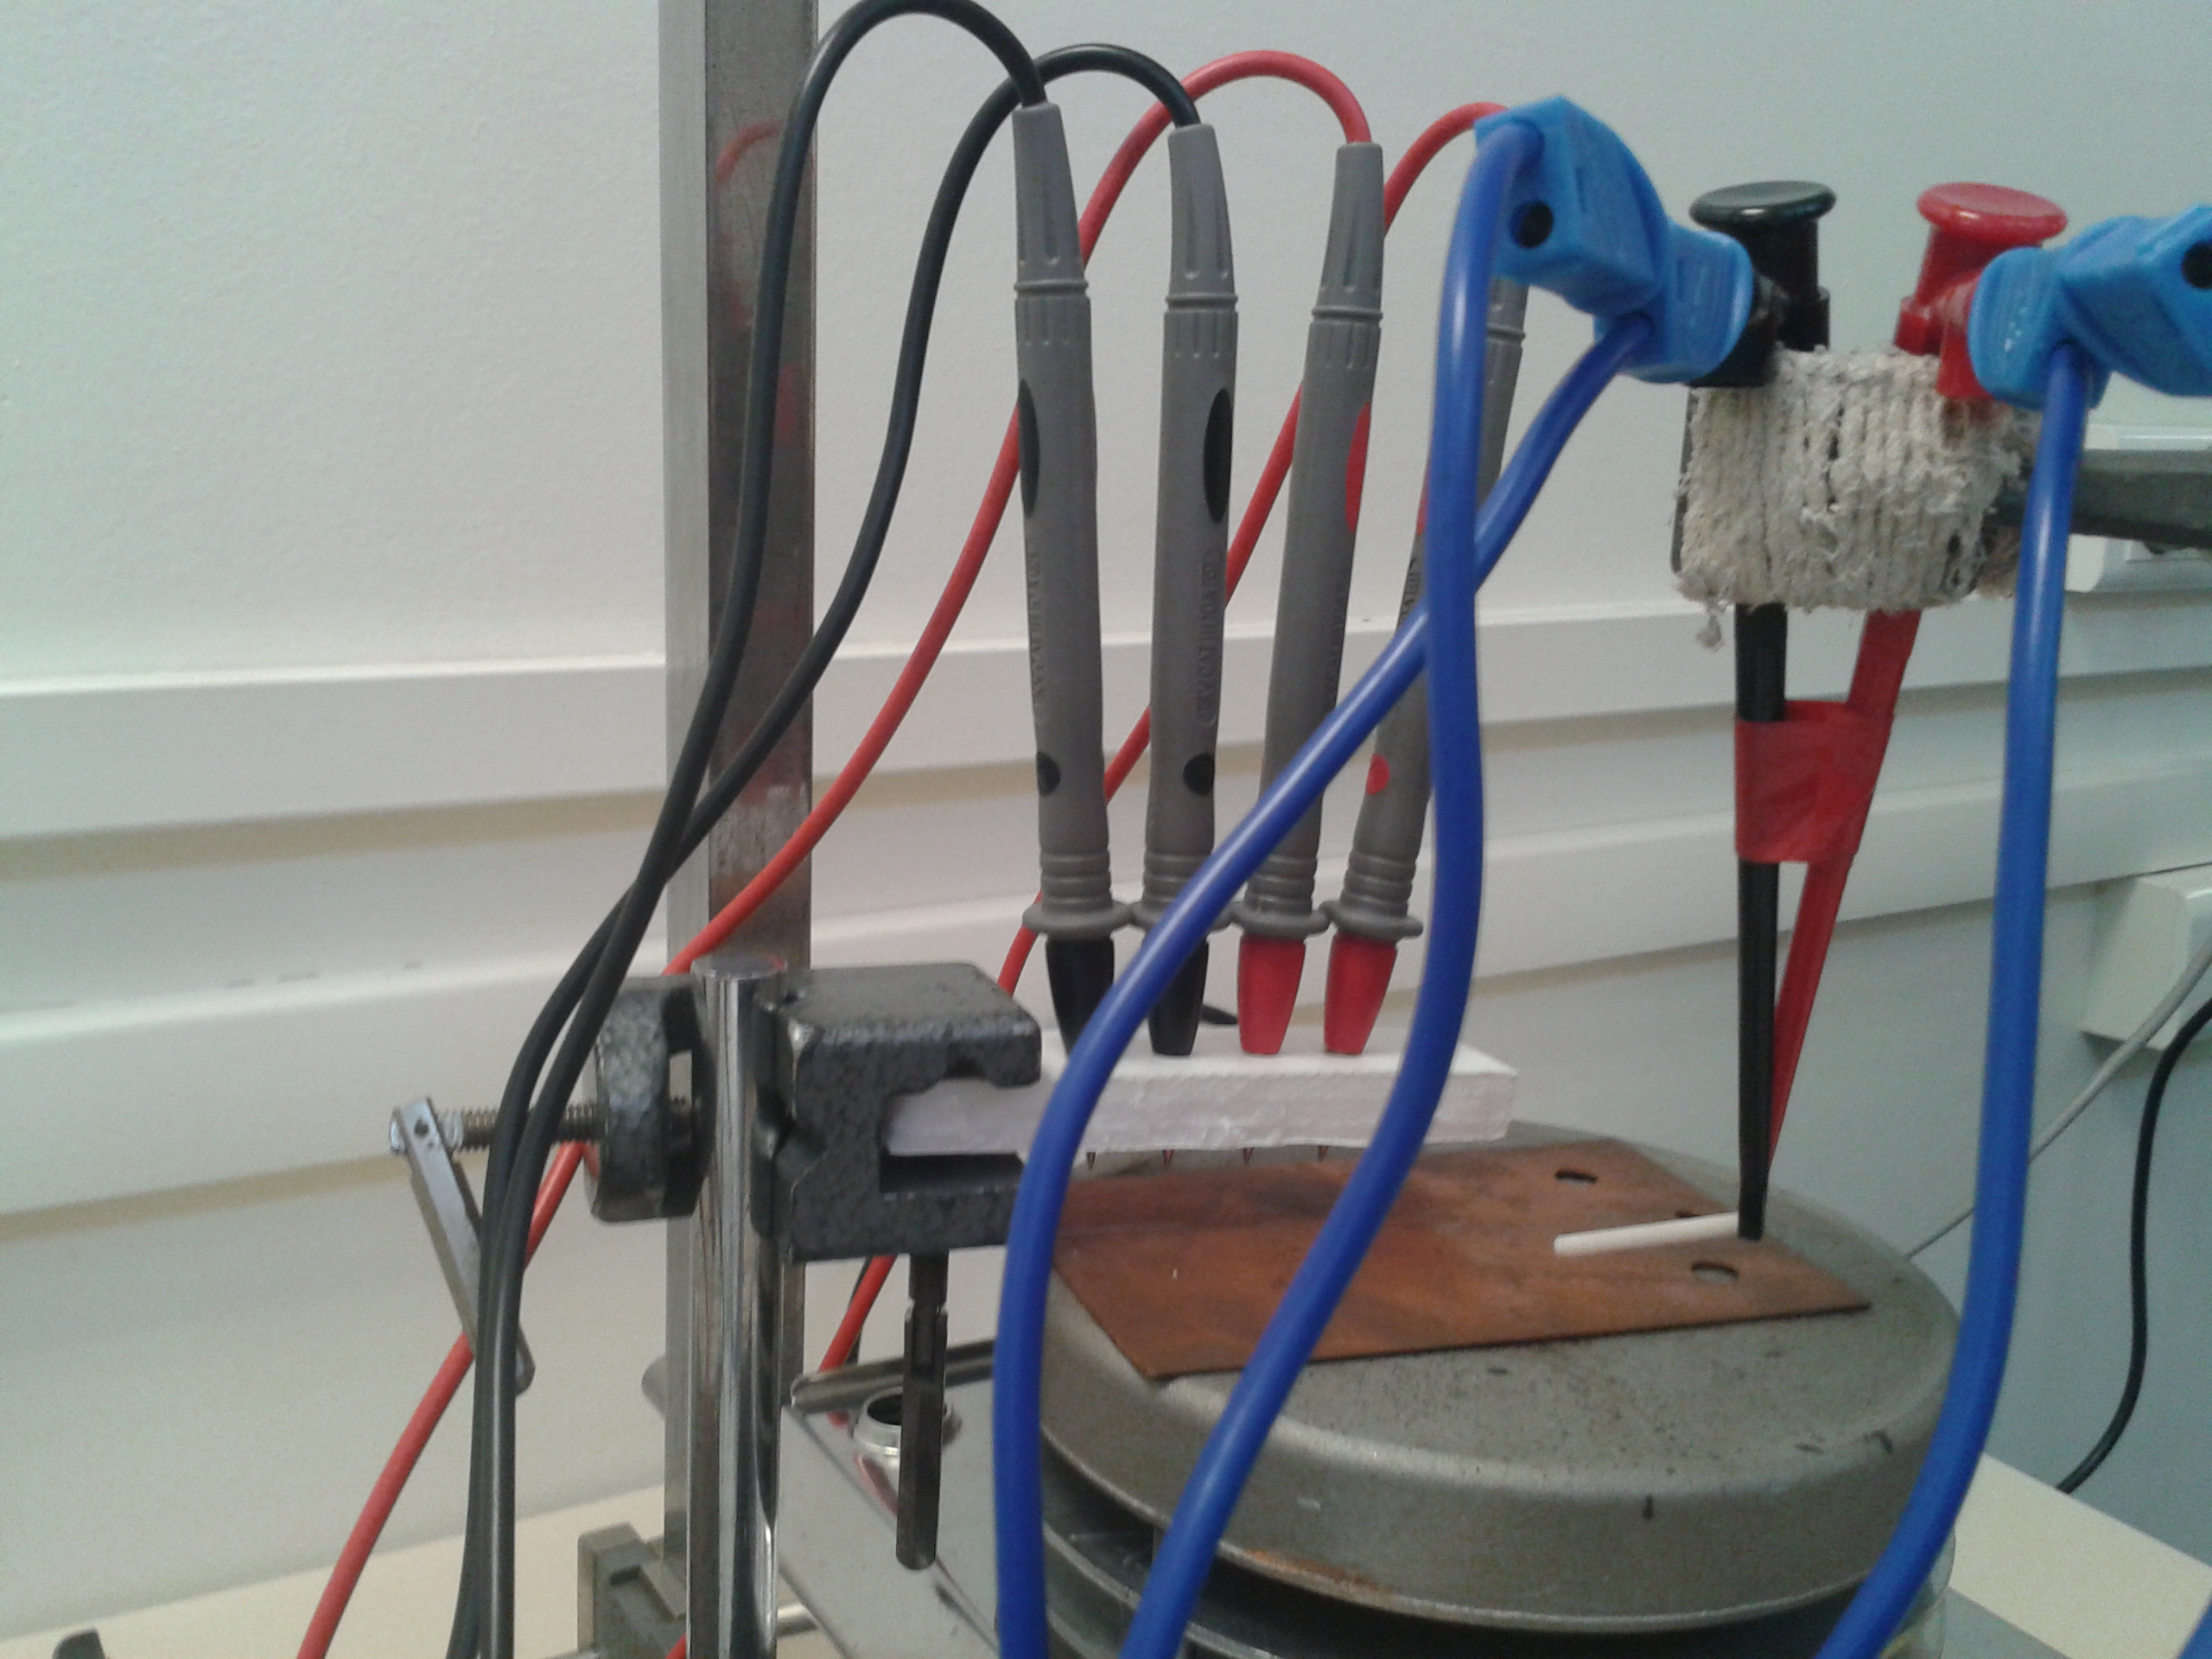
\includegraphics[width=10cm]{./images/photo2.jpg}
		\caption{Gros plan sur les sondes de mesure de résistance et de température}
		\label{photo2}
	\end{center}
\end{figure}
\begin{figure}[!t]
  \begin{center}
		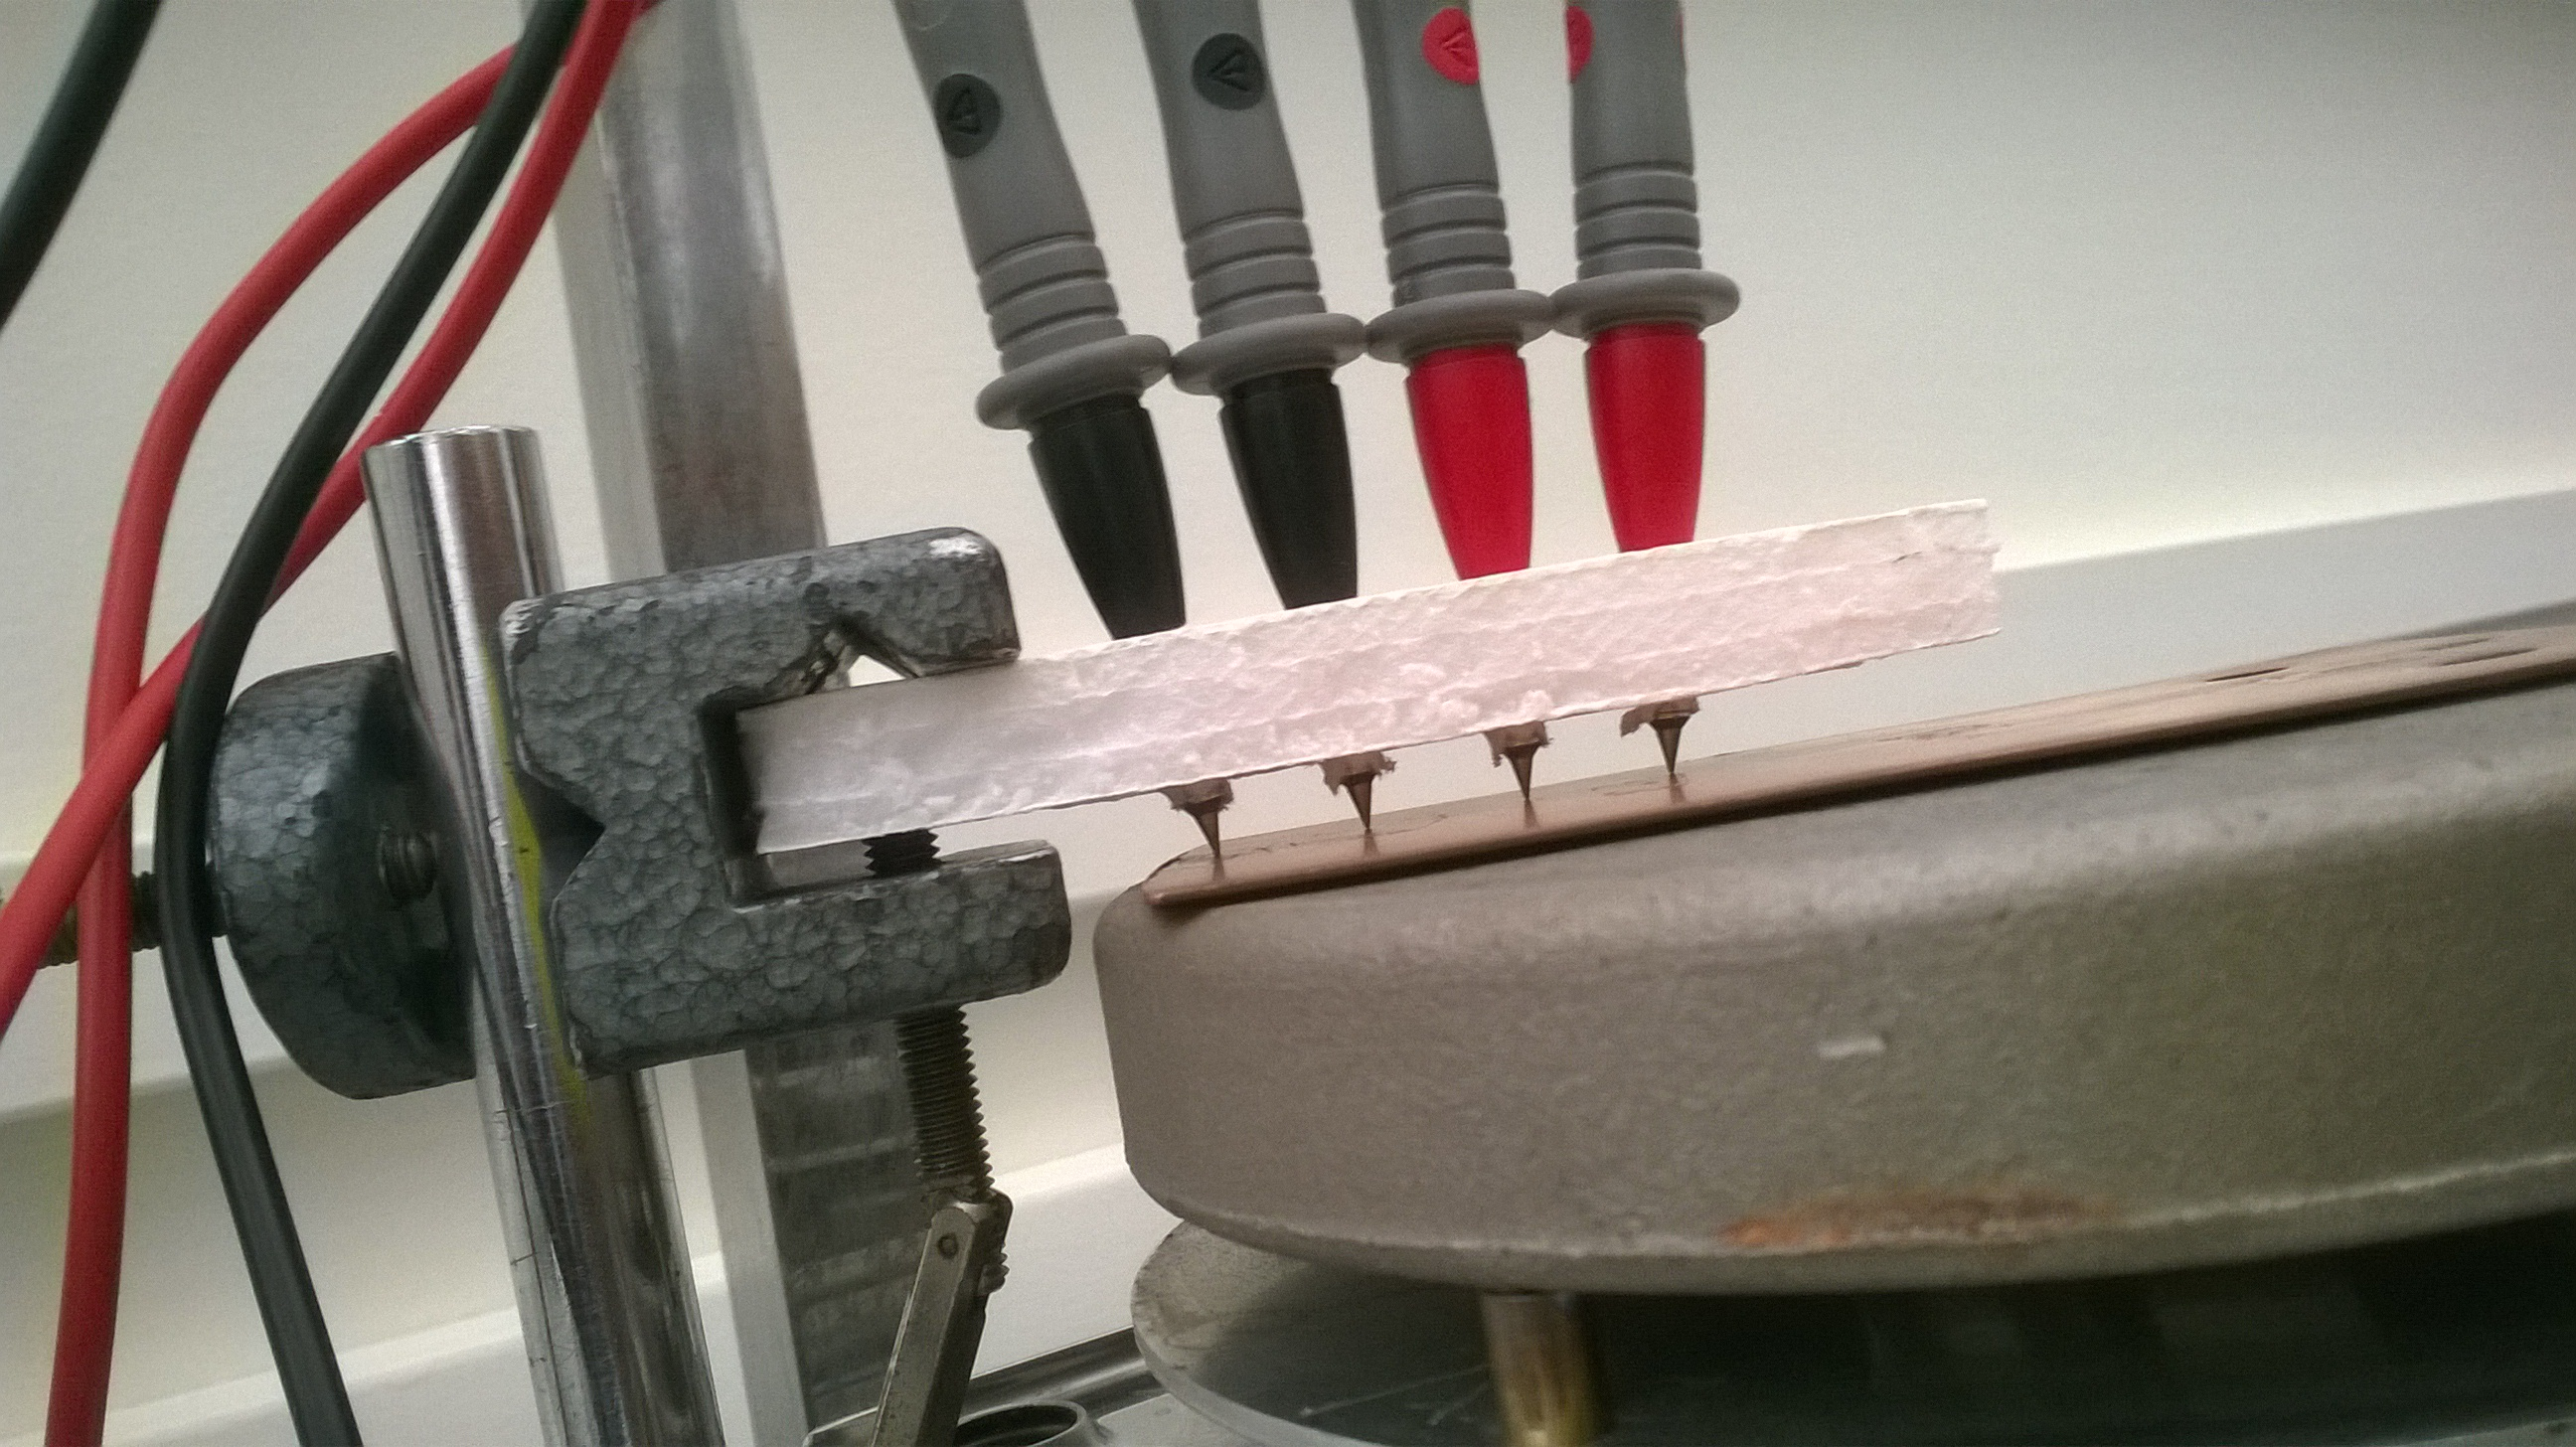
\includegraphics[width=10cm]{./images/photo3.jpg}
		\caption{Les 4 pointes en contact}
		\label{photo3}
	\end{center}
\end{figure}

\newpage

Enfin, sur les 2 photos suivantes : Figures \ref{photo4} et \ref{photo5}, on peut voir le porte-échantillon rempli de billes de verre, et dans lequel est inséré la sonde de température, ce montage étant utilisé dans le cas du refroidissement à l'azote liquide (on verse l'azote dans ce porte-échantillon adapté à ce type de manipulations à très basse température.

\begin{figure}[!b]
  \begin{center}
		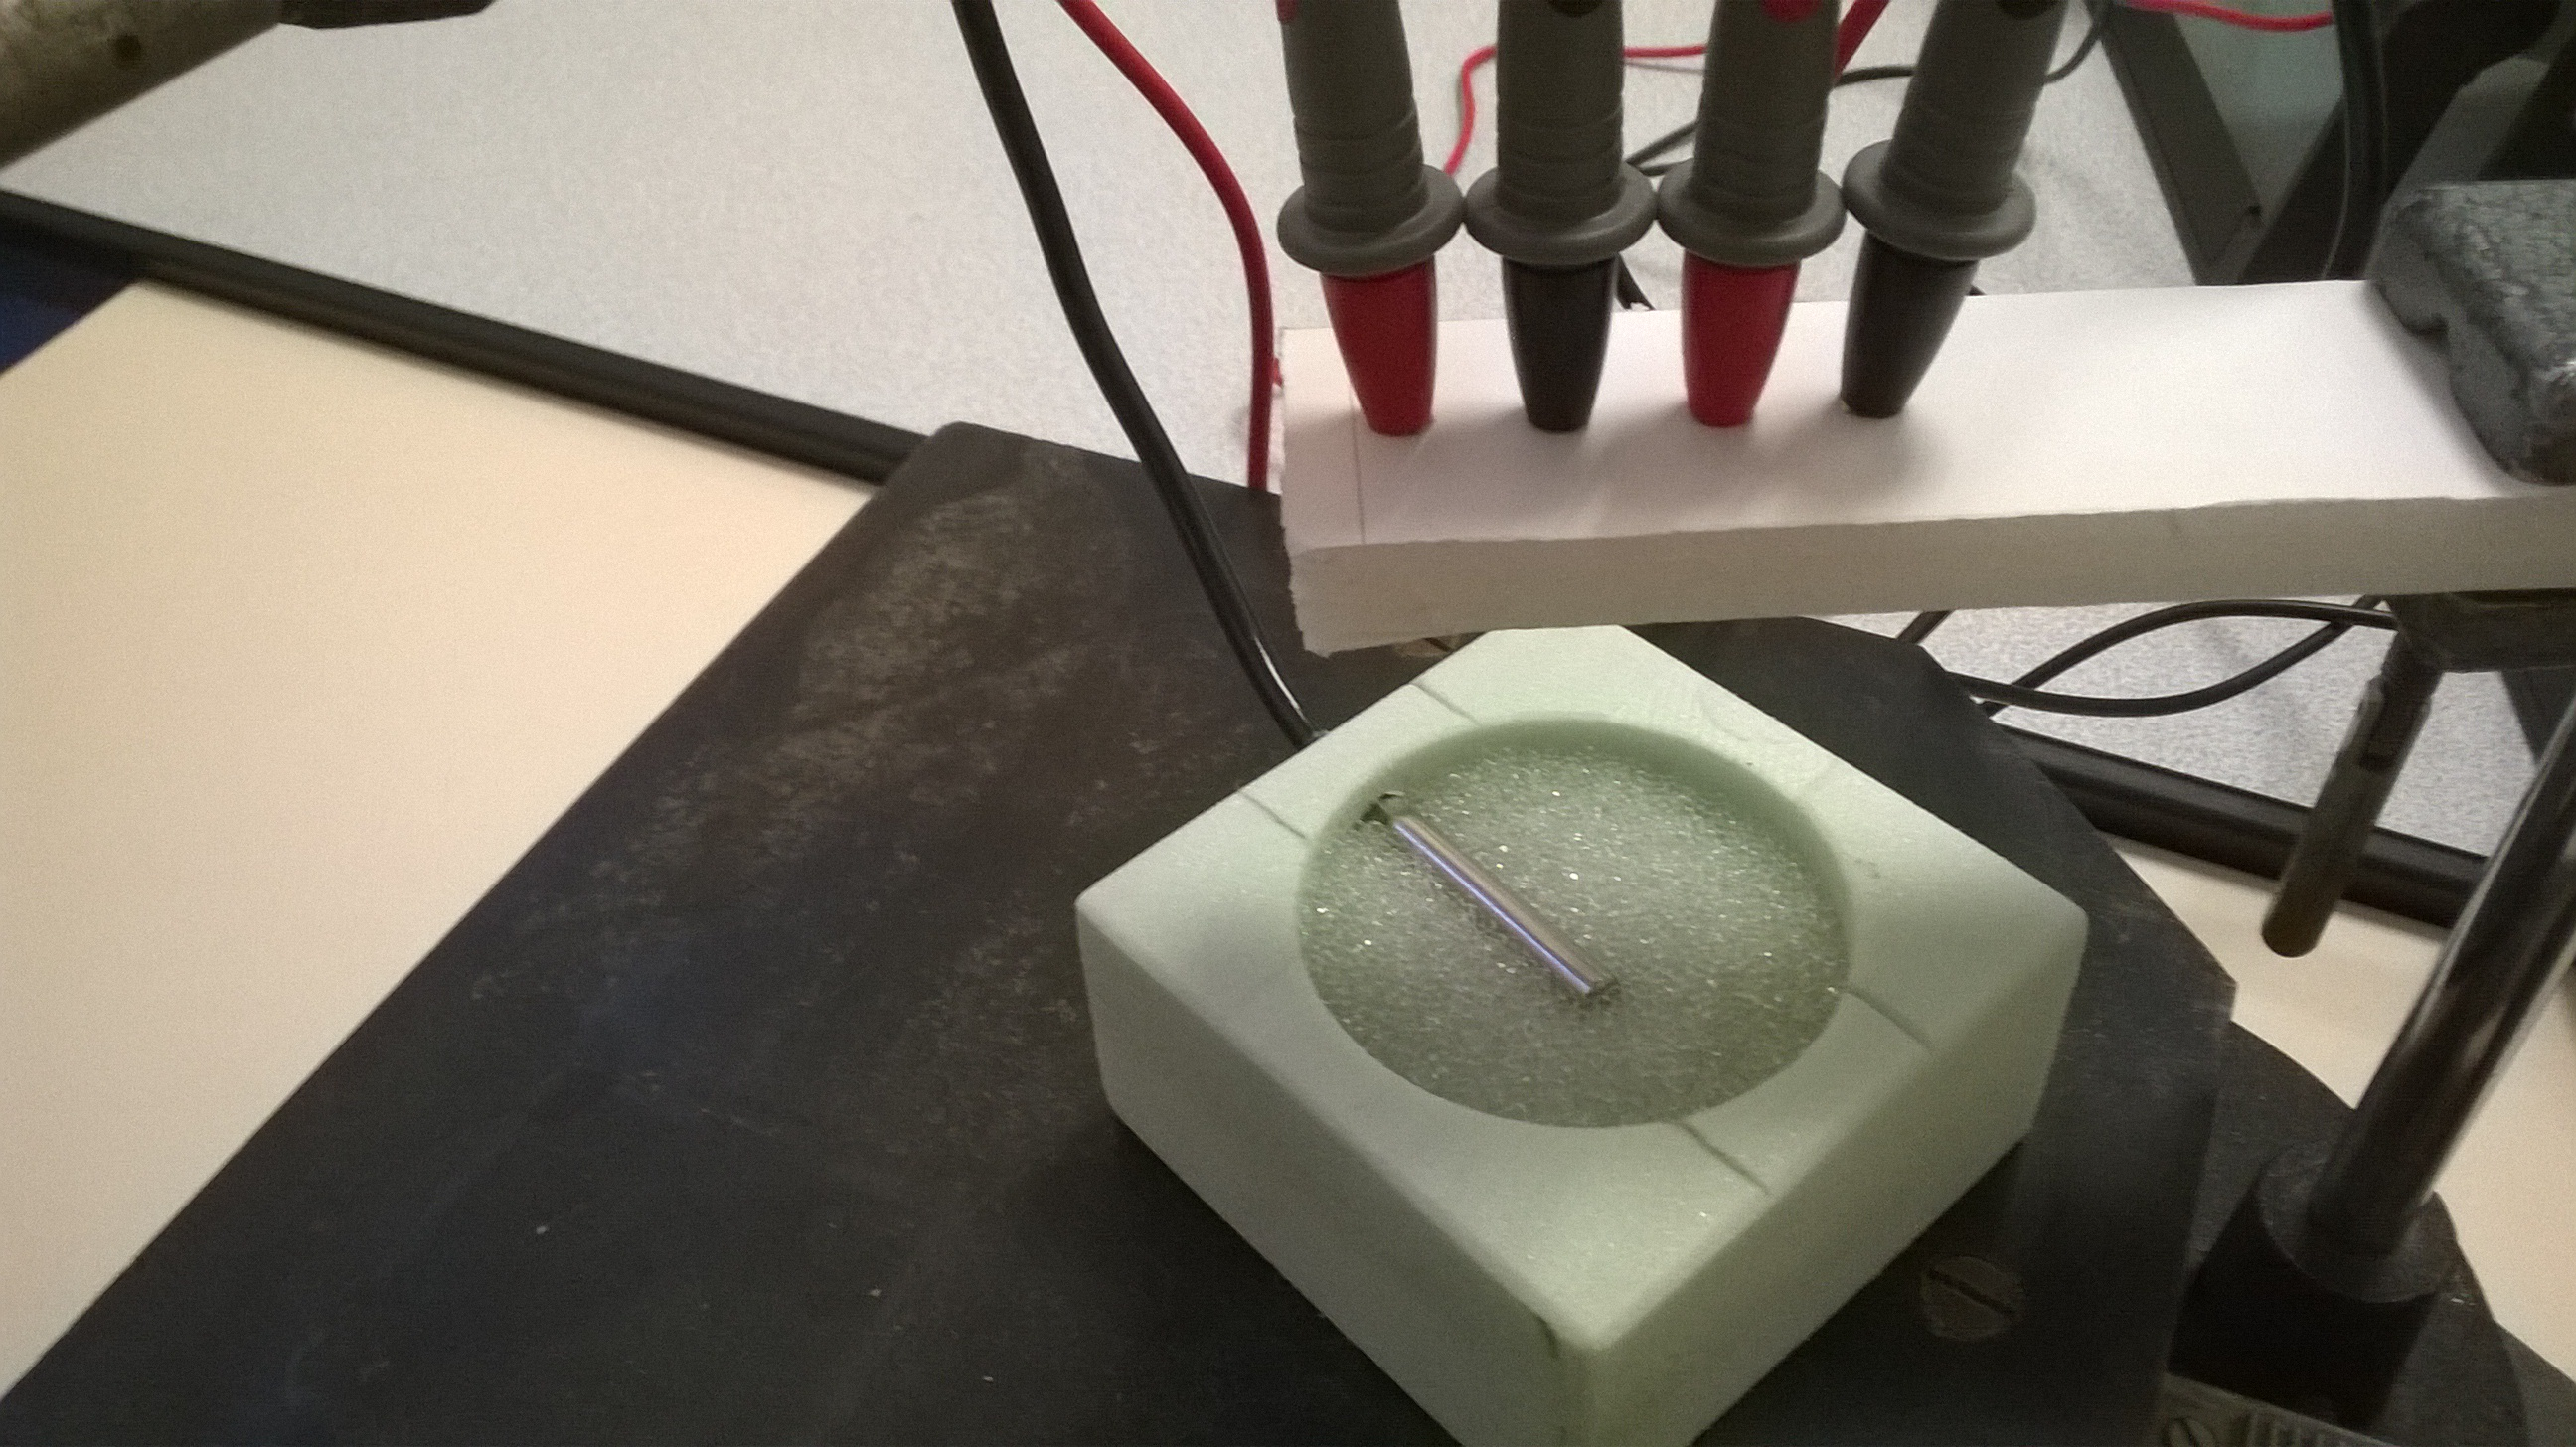
\includegraphics[width=10cm]{./images/photo4.jpg}
		\caption{Porte-échantillon pour le refroidissement à l'azote liquide}
		\label{photo4}
	\end{center}
\end{figure}
\begin{figure}[!t]
  \begin{center}
		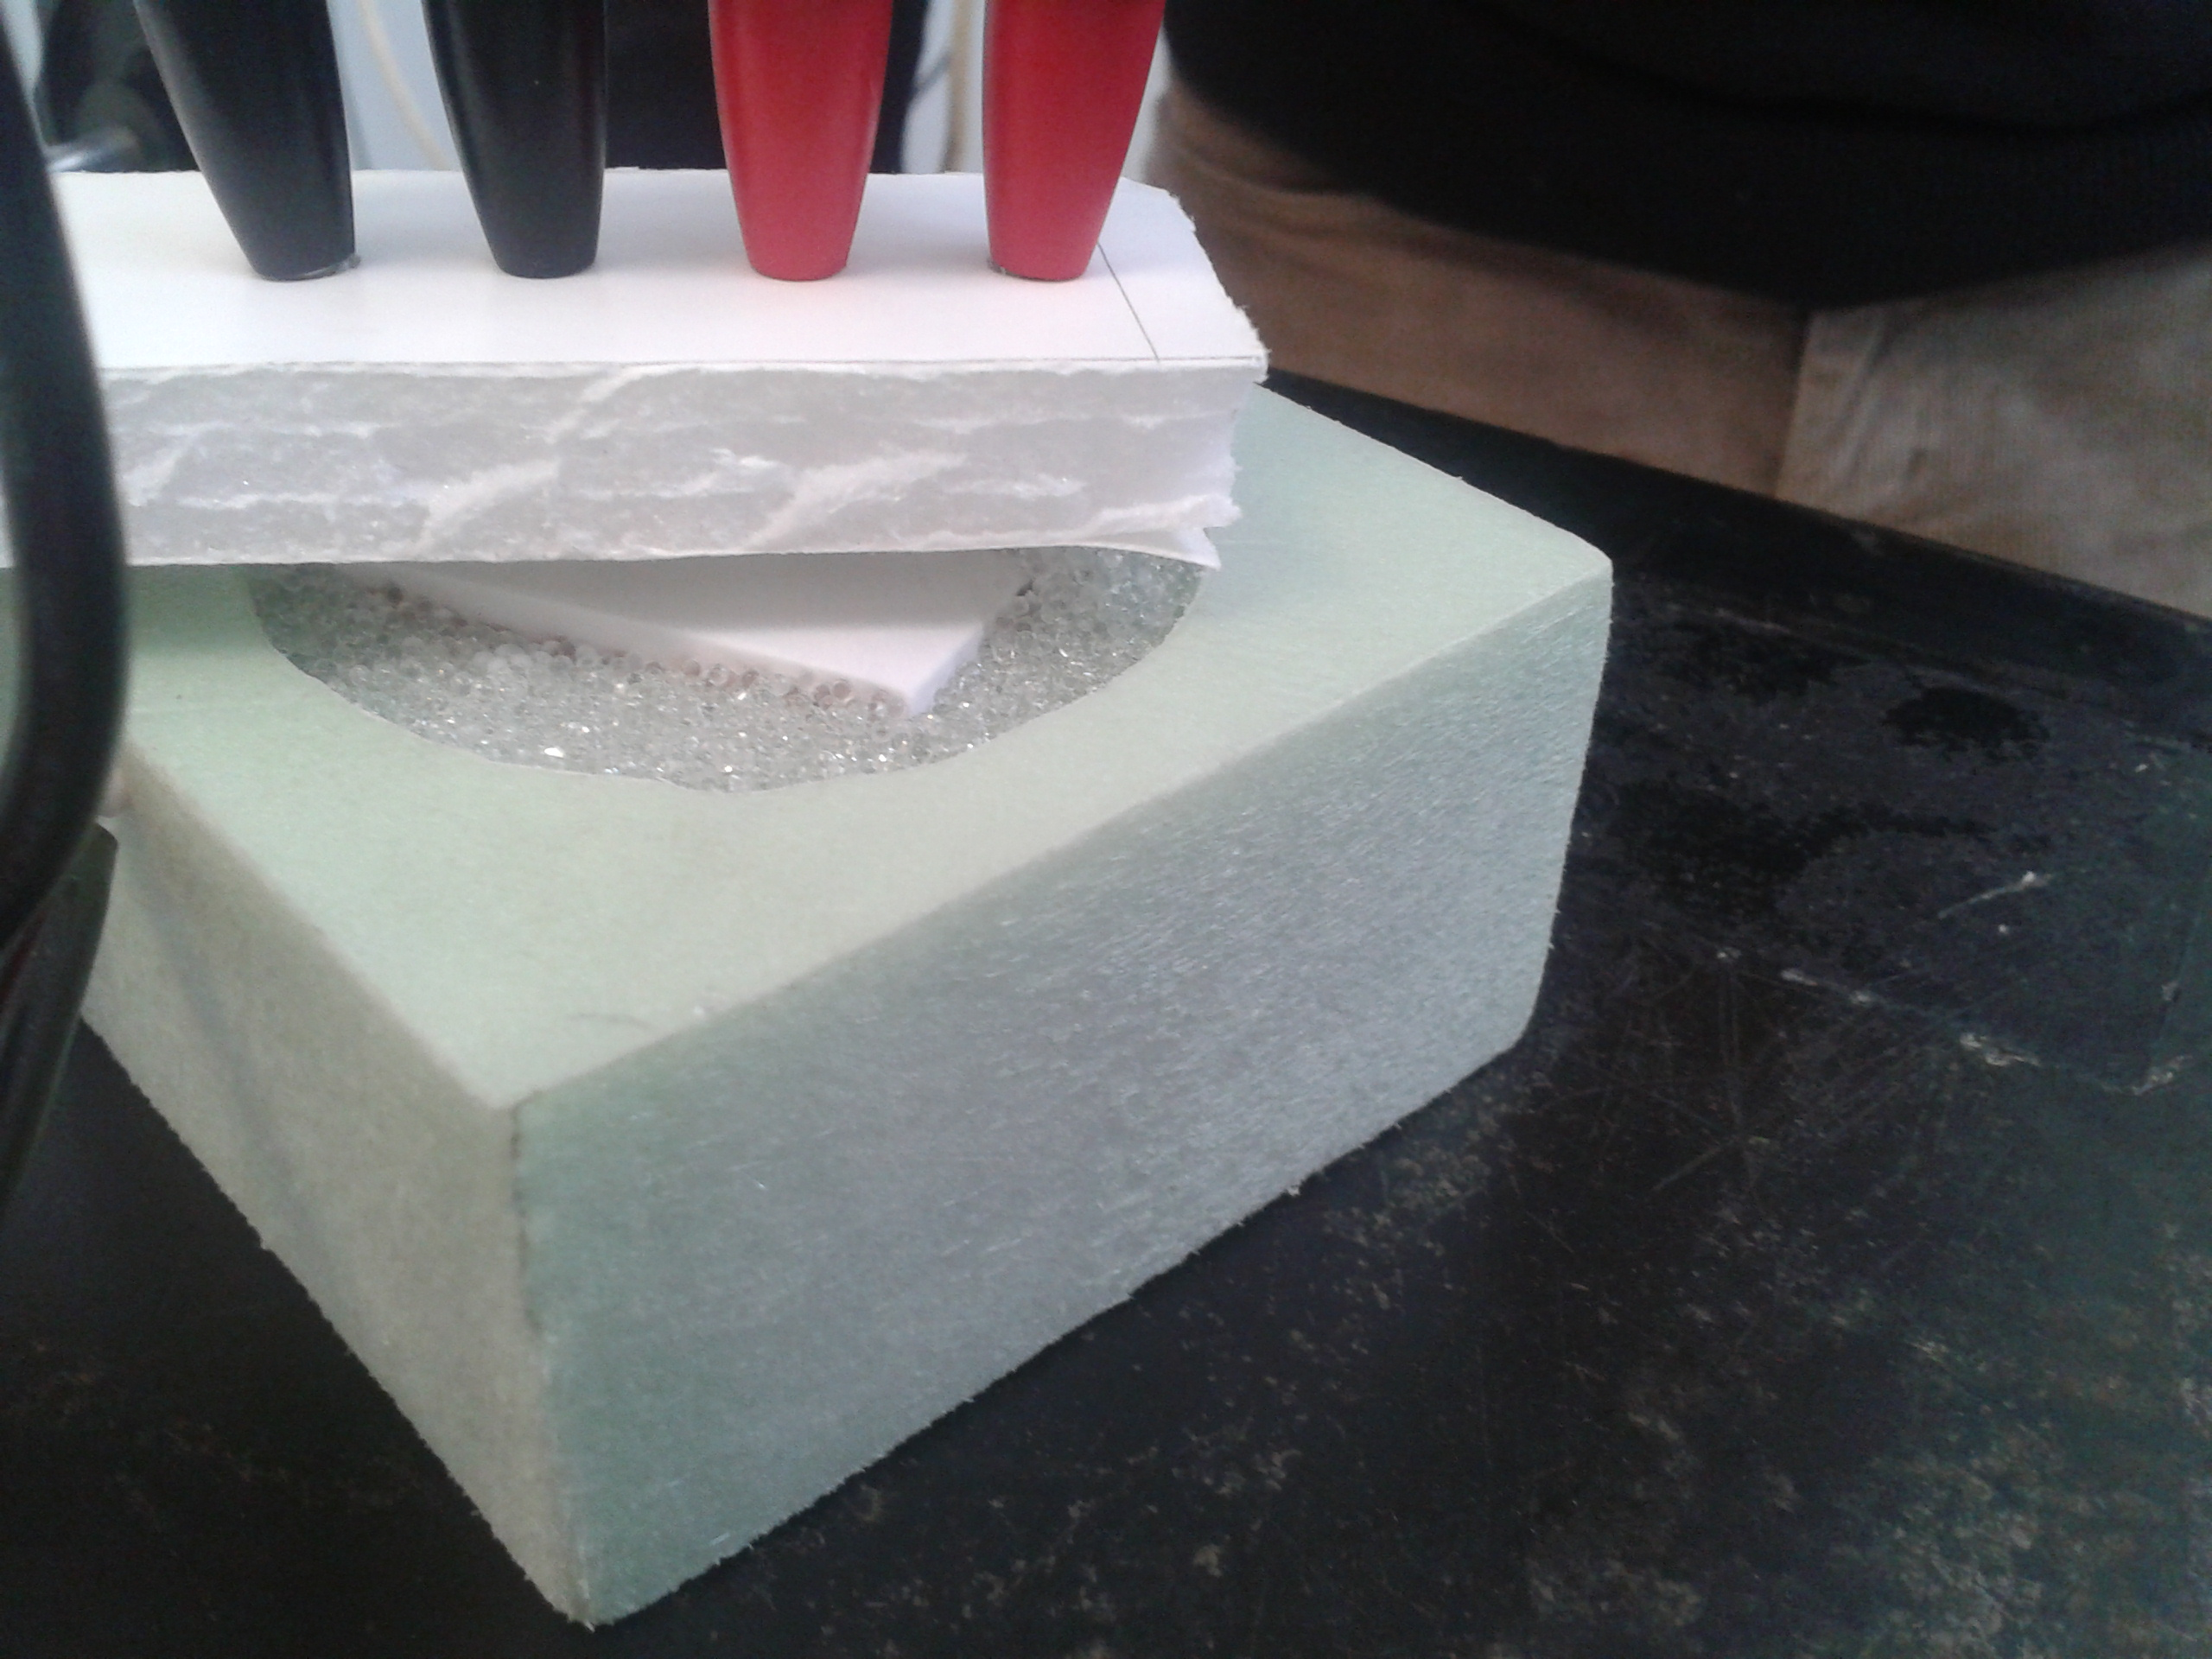
\includegraphics[width=10cm]{./images/photo5.jpg}
		\caption{Les 4 pointes en contact au cours d'une mesure avec refroidissement à l'azote liquide}
		\label{photo5}
	\end{center}
\end{figure}

\newpage

\subsection{Conditions expérimentales}
Nous avons utilisé Labview pour réaliser les acquisitions des deux résistances mesurées.
Nous avons simplement posé la plaque de cuivre sur une plaque chauffante et mesuré sa résistance en fonction de la température en 4 pointes, entre 25\celsius{} et 205\celsius{}.


Pour le silicium, nous voulions détecter un palier de conductivité (car il s'agissait d'échantillons dopés), et nous savions que ce palier risquait de se trouver à une température inférieure ou égale à la température ambiante.
Donc, pour pouvoir étudier ce palier, nous avons dû baisser fortement la température et nous avons utilisé de l'azote liquide pour cela.
Nous avons également placé des billes de verre dans notre porte-échantillon pour augmenter l'inertie thermique du montage et nous permettre d'avoir une montée en température relativement lente.
La sonde de température a été insérée dans le porte-échantillon par un trou percé sur le côté (voir montage). De cette façon, elle peut être en contact du silicium et être entourée par les billes de verre.
De ce fait, elle mesure bien mieux la température du silicium que si on l'avait simplement posée dessus.


\paragraph{Pourquoi une mesure 4 pointes (et pas tout simplement 2) ?}
La mesure 4 pointes consiste à injecter un courant avec deux pointes et à mesurer une tension avec deux autres placées entre les deux premières.
Cette méthode permet de s'affranchir des résistances des fils et des résistances de contact.
Elle est donc particulièrement utile pour mesurer des résistances de l'ordre de l'$\Omega$ ou inférieures, car c'est l'ordre de grandeur des résistances parasites.
Par contre, elle est parfaitement inutile pour les hautes résistances (plusieurs k$\Omega$, M$\Omega$), donc on aurait mesuré en 2 pointes pour un isolant par exemple.


\paragraph{Principe de la sonde, comment a-t-on étalonné la sonde ?}
Nous avons étalonné la sonde Pt en deux étapes :


\begin{itemize}
  \item en la plaçant dans de l'eau que nous avons fait bouillir, nous avons pu mesurer la résistance de la sonde à une température de 100\celsius{}.
  \item en la plaçant ensuite dans de l'eau pleine de glaçons, nous avons fait la même chose pour 0\celsius{}.
\end{itemize}


La résistance du platine augmente linéairement avec la température, c'est une propriété de ce matériau.
On obtient alors la caratéristique R(T) : en mesurant la résistance du Platine, on peut en déduire sa température (donc idéalement la température de l'échantillon).


\paragraph{Interfaçage grâce à Labview}
L'utilisation de l'outil informatique pour mener à bien l'expérience était prévu pour cet AE 
et en constituait une des principales caractéristiques. En effet notre encadrant nous avait fortement recommandé 
d'automatiser les mesures pour faciliter la prise de donnée tout en gagnant du savoir faire expérimental. L'outil de 
prédilection pour ce type de mesure est le logiciel LabVIEW qui permet de réaliser l'acquisition des données. 
Nous avons donc décidé d'utiliser ce logiciel. Le but était de pouvoir contrôler les deux flukes avec l'ordinateur. 
La prise de données par voie informatique comporte trois volets que nous avons du nous approprier successivement : 

\begin{enumerate}
\item la connection des appareils à l'ordinateur ; 
\item leur reconnaissance par ce dernier ; 
\item et le codage du code LabView. 
\end{enumerate}

La première étape a été réalisée grâce à deux cables smart488, dont l'un des deux qu'il a fallu commander. 
Ces câbles permettent le passage d'une sortie GPIB à une sortie USB et possèdent un contrôleur intégré. 
C'est ce contrôleur qu'il a fallu régler, grâce à un logiciel dédié, pour pouvoir détecter les deux flukes 
par l'ordinateur. On a aussi utilisé le logiciel NiMax pour vérifier la compatibilité avec Labview. 
Après cela on a entamé l'étape d'écriture du code graphique Labview. Ce code devait nous permettre d'acquérir 
simultanément, et dans le temps, les signaux des deux multimètres, qui correspondent à la température de la sonde 
et à la résistance de l'échantillon. L'acquisition se fait pendant un laps de temps prédéfini. Les résultats obtenus sont présentés sous forme de tableau qui peut être lisible par un logiciel comme gnuplot.
[Ajouter photo du code et de la "face avant" de labview + photo cable smart488]


\subsection{Difficultés expérimentales}
Deux principales difficultées expérimentales se sont posées lors de cette activité expérimentale. 
Tout d'abord il y a eu le problème de l'automatisation des résultats et de l'interfaçage avec l'ordinateur.
On a eu du mal à réaliser chacune des trois étapes reliées à l'automatisation des mesures, mais plus particulièrement 
pour la détection des instruments par l'ordinateur parce que cela mettait en jeu différents composants tels que le 
multimètre, le cable smart488 et labview.

D'autre part le contact entre les électrodes et l'échantillon s'avéra bien plus délicat que prévu. 
En effet l'utilisation du montage à quatre pointes oblige à avoir quatre contacts stables. On a donc implémenté 
le montage tel qu'il apparait dans la figure [figure du montage]. Le premier essai sur le cuivre donna des résultats 
très cohérents mais les essais sur les échantillons de silicium donnaient des valeurs très instables. 
En effet la valeur de la résistance changeait de plusieurs ordres de grandeurs selon la pression exercée sur les 
pointes. On soupçonnait les fils ou les pointes d'être a l'origine de ces fluctuations 
mais on compris plus tard que cela était probablement dû à l'hétérogénité de la surface de l'échantillon de silicium. 
En effet le silicium au contact de l'air s'oxyde et on obtient une couche de SiO2 à la surface de l'échantillon. 
La variation de la résistance selon la pression exercée sur les pointes peut donc provenir du fait que la pointe 
traverse où pas cette couche. Cependant lorsque on exerce une pression constante on obtient des résultats cohérents avec la nature semiconductrice du silicium comme on pourra le voir dans nos résultats. Une façon d'obtenir cette pression constante et donc un meilleur contact est d'utiliser des pointes avec à ressorts fixées solidement au support. Cependant on a pas pu se procurer de tels contacts avant la fin de l'activité et nous avons du réaliser plusieurs fois la même éxpérience jusqu'à obtenir une valeur stable.

% /!\ non je ne pense pas que ce soit ça, c'est bien les contacts qui se modifient au cours du temps 
% (à cause de la chaleur...). On parle de l'idée des ressorts pour améliorer ça ?

\subsection{Résultats}
Pour le cuivre, nous avons simplement observé que la conductivité diminue quand on augmente la température (voir courbe).
[donner un ordre de grandeur de la conductivité du cuivre sur cette plage de température si elle est bonne]


Pour le silicium, nous avons observé une conductivité croissante avec la température, ce qui est cohérent. Nous avons aussi observé un palier aux alentours de [20\celsius{}; 80\celsius{}], ce qui semble cohérent aussi.
À haute température, on observe à nouveau une croissance de la conductivité, 
puis les contacts se sont dégradés donc on n'a pas pu monter plus haut en température.


\subsubsection*{Tableaux}

\subsubsection*{Courbes}


\subsection{Discussion des résultats}

L'endroit où se trouve le palier paraît cohérent, pour le Si il est autour de la température ambiante, c'est pourquoi le Si est utilisé dans l'électronique.


%(c'est ce qu'on avait noté pour l'oral) : 
%Pour le fait qu'on identifie qu'il s'agit d'un échantillon dopé je parle des différentes allures de conductivités en fonction de T dans ma partie, on se raccrochera à ça.
%Pour la détermination du dopage, il faut repérer la conductivité de notre échantillon de Si à Tamb et à l'aide d'abaques en déduire le dopage (j'ai vite fait essayé, sans valeurs de conductivités précises, et je trouve un dopage de 10^20 porteurs par cm^3)
%[double plateau, essaye de lire sur wiki pour bien comprendre on risque d'avoir des questions dessus/ le type de dopage n'est pas visible directement, peut etre en faisant un truc special avec la vitesse des porteurs mais je ne crois pas]]


\subsection{Conclusions}

